\documentclass{article}

\usepackage{amsmath}
\usepackage{amssymb}
\usepackage{amsfonts}
\usepackage{mathtools}

\usepackage{fullpage}

\usepackage{ wasysym }

\usepackage[thmmarks, amsmath]{ntheorem}

\usepackage{graphicx}
\usepackage{float}
\usepackage{tikz-cd}
\usepackage{adjustbox}

\usepackage{diffcoeff}
\difdef{f}{}{
outer-Ldelim = \left. ,
outer-Rdelim = \right| ,
sub-nudge = 0 mu
}
\difdef{f}{p}{
op-symbol = \mathrm{D},
op-symbol-alt = \mathrm{d}
}

\usepackage{cancel}
\usepackage{interval}

\usepackage{array}

\usepackage{enumitem}

\setlist[enumerate,1]{label=(\alph*)}

\title{Differential Geometry Homework 4}
\author{Duarte Maia}
%\date{}

\theoremstyle{plain}
\theorembodyfont{\upshape}
\theoremseparator{.}
\newtheorem{theorem}{Theorem}
\newtheorem{prop}{Prop}
\renewtheorem*{prop*}{Prop}
\newtheorem{lemma}{Lemma}
\newtheorem*{ex}{Exercise}

\theoremstyle{nonumberplain}
\theoremheaderfont{\itshape}
\theorembodyfont{\upshape}
\theoremseparator{:}
\theoremsymbol{\ensuremath{\blacksquare}}
\newtheorem{proof}{Proof}
\newtheorem{sol}{Solution}

\theoremsymbol{\text{\textit{(End proof of lemma)}}}
\newtheorem{lemmaproof}{Proof of lemma}

\newcommand{\R}{\mathbb{R}}
\newcommand{\C}{\mathbb{C}}
\newcommand{\Z}{\mathbb{Z}}
\newcommand{\Q}{\mathbb{Q}}

\newcommand{\RP}{\mathbb{RP}}
\newcommand{\HH}{\mathbb{H}}

\newcommand{\kk}{\Bbbk}

\newcommand{\PP}{\mathbb{P}}
\newcommand{\FF}{\mathcal{F}}

\newcommand{\I}{\mathrm{i}}
\newcommand{\e}{\mathrm{e}}

\newcommand{\id}{\mathrm{id}}
\newcommand{\GL}{\mathrm{GL}}
\newcommand{\SO}{\mathrm{SO}}
\newcommand{\SL}{\mathrm{SL}}

\newcommand{\conj}[1]{\overline{#1}}
\newcommand{\close}[1]{\overline{#1}}
\newcommand{\into}{\mathbin{\lrcorner}}

\DeclareMathOperator{\interior}{int}
\DeclareMathOperator*{\colim}{colim}
\DeclareMathOperator{\codim}{codim}
\DeclareMathOperator{\trace}{tr}
\DeclareMathOperator{\Lie}{L}
\newcommand{\grad}{\nabla}
\newcommand{\transp}{\top}
\DeclareMathOperator{\tg}{tg}


\let\Diff\relax
\DeclareMathOperator{\Diff}{Diff}
\DeclareMathOperator{\Ext}{Ext}
\DeclareMathOperator{\Hom}{Hom}

\let\div\relax
\DeclareMathOperator{\div}{div}

\DeclarePairedDelimiter{\abs}{\lvert}{\rvert}
\DeclarePairedDelimiter{\norm}{\lvert}{\rvert}
\DeclarePairedDelimiter{\Norm}{\lVert}{\rVert}
\DeclarePairedDelimiter{\braket}{\langle}{\rangle}


\begin{document}
\maketitle

\begin{ex}[\#11 from do Carmo]
Prove that the divergence satisfies
\begin{equation}
\dl(X \into \nu) = (\div X) \nu.
\end{equation}
\end{ex}

\begin{sol}
Since the space of $n$-forms is one-dimensional, it suffices to prove that $\dl(X \into \nu) = (\div X) \nu$ on a chosen basis of $T_p M$. Thus, pick an orthonormal basis $e_1, \dots, e_n$ of $T_p M$, and extend it to an orthonormal frame $E_1, \dots, E_n$ around $p$. Then, by a known formula for the exterior product, we have
\begin{equation}
\dl(X \into \nu)(e_1, \dots, e_n) = \sum_i (-1)^{i+1} e_i \cdot \nu(X, E_{\hat\imath}),
\end{equation}
where $E_{\hat\imath}$ means $E_1, \dots, E_n$ with the $i$-th place removed.

Now, it is easy to check that, by skew-linearity, and setting $X = \sum_j g(X, E_j) E_j$,
\begin{equation}
(-1)^{i+1} \nu(X, E_{\hat\imath}) = (-1)^{i+1} \nu(g(X, E_i) E_i, E_{\hat\imath}) = g(X,E_i) \nu(E_1,\dots,E_n) = g(X,E_i).
\end{equation}
As a consequence, we have
\begin{equation}
\dl(X \into \nu)(e_1, \dots, e_n) = \sum e_i \cdot g(X,E_i),
\end{equation}
which is in turn equal to $\left(\sum g(\nabla_{E_i} X, E_i)\right) + \left( \sum_i g(X, \nabla_{E_i} E_i) \right)$. The first term is precisely $\div X$, or equivalently $(\div X) \nu(E_1, \dots, E_n)$. Thus, we seek to prove that the second term equals zero.

To do this, we make use of the fact that we have not yet specified the construction of the frame $E_i$ around $p$. Thus, we have the freedom to ensure that $E_i$ is parallel along the geodesic that starts at $p$ with velocity $e_i$, which in turn will guarantee that $(\nabla_{E_i} E_i)_p = 0$. This completes the proof.
\end{sol}

\pagebreak

\begin{ex}[\#12 from do Carmo]
(The following is protected by the First Amendment, which protects parody under the umbrella of Free Use.)
\end{ex}
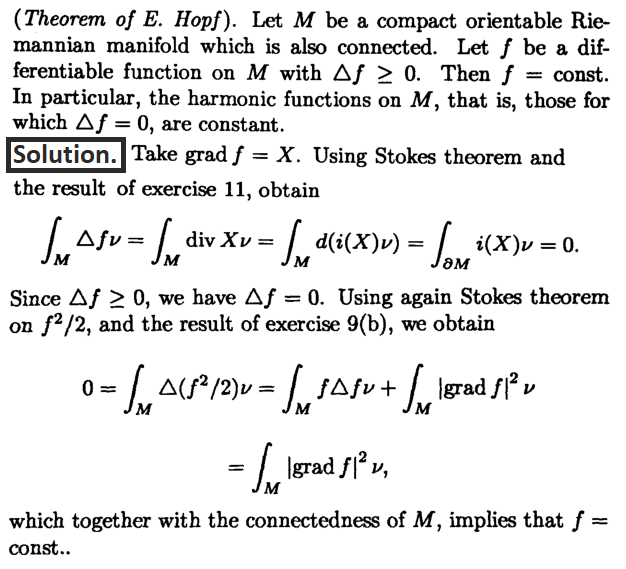
\includegraphics[width=\linewidth]{hint}

\begin{ex}[\#13 from do Carmo]
Let $\nu = f \dl x_1 \wedge \dots \wedge \dl x_n$, and $X = \partial_{x_1}$. Show that $X \into \nu = f \dl x_2 \wedge \dots \wedge \dl x_n$.

Conclude that $\div X = \frac1f \partial_{x_1} f$.
\end{ex}

\begin{sol}
The first part is obvious from the definition of wedge, and the fact that $(\dl x_i) X = \delta_{i1}$. For the second part, we note that
\begin{equation}
\dl(X \into \nu) = \dl f \wedge \dl x_2 \wedge \dots \wedge \dl x_n = (\partial_{x_1} f) \dl x_1 \wedge \dots \wedge \dl x_n = \frac1f (X \cdot f) \nu,
\end{equation}
where the second equality uses the decomposition $\dl f = \sum \partial_{x_i} f \, \dl x_i$. Anyhow, by applying exercise 11, we immediately obtain the desired equality.
\end{sol}

\begin{ex}[\#1 from do Carmo]
\leavevmode
\begin{enumerate}
\item Show that $\nabla_X Y = \frac12 [X,Y]$.
\item Conclude that $R(X,Y) Z = \frac14 [[X,Y],Z]$.
\item Prove that if $X$ and $Y$ are orthonormal, we have
\begin{equation}
K(\sigma) = \frac14 \Norm{[X,Y]}^2.
\end{equation}
\end{enumerate}
\end{ex}

\begin{sol}
\leavevmode
\begin{enumerate}
\item We expand $\nabla_{X+Y} (X+Y) = 0$, which gets us (together with torsion freeness):
\begin{equation}
0 = \nabla_X Y + \nabla_Y X = 2 \nabla_X Y - [X,Y],
\end{equation}
and we have the result.

\item We expand: $R(X,Y) Z = \nabla_X \nabla_Y Z- \nabla_Y \nabla_X Z - \nabla_{[X,Y]} Z$, and it follows:
\begin{equation}
\begin{aligned}
\nabla_X \nabla_Y Z- \nabla_Y \nabla_X Z - \nabla_{[X,Y]} Z &=
\frac14 [X, [Y, Z]] - \frac14 [Y, [X,Z]] - \frac12 [[X,Y],Z]\\
&= \frac14 [X, [Y, Z]] + \frac14 [Y, [Z,X]] - \frac12 [[X,Y],Z]\\
&= -\frac14 [Z, [X,Y]] + \frac12[Z,[X,Y]] = -\frac14 [[X,Y],Z].
\end{aligned}
\end{equation}

This is right up to sign.
\item Write for $X$, $Y$ orthonormal $K(\sigma) = \braket{R(X,Y) X, Y}$. By previous exercise, and the formula $\braket{[U,X], V} = - \braket{U,[V,X]}$ which we saw in a previous homework,
\begin{equation}
K(\sigma) = -\frac14 \braket{[[X,Y], X], Y} = \frac14 \Norm{[X,Y]}^2.
\end{equation}
\end{enumerate}
\end{sol}

\begin{ex}[3]
\leavevmode
\begin{enumerate}
\item Show that $g$ is harmonic wrt $\braket{,}$ iff it is harmonic wrt $\braket{,}^E$.
\item Show that $k_p = -\frac12 \frac{\Delta(\log \rho)}{\rho^2}$.
\end{enumerate}
\end{ex}

\begin{sol}
\leavevmode
\begin{enumerate}
\item We apply the formula for the Laplacian in terms of the metric tensor:
\begin{equation}
\Delta f = \sum_k \frac1{\sqrt{\det(g_{ij})}} \partial_k \left( \sqrt{\det(g_{ij})} \sum_\ell g^{k \ell} \partial_\ell f \right)
\end{equation}
and note that in our case, $g_{ij} = \rho^2 \delta{ij}$, hence the determinant is $\rho^4$ and its square root is $\rho^2$. Moreover, $g^{ij} = \rho^{-2} \delta_{ij}$, so the above formula reduces to
\begin{equation}
\Delta f = \rho^{-2} \sum_k \partial_k \left( \rho^2 \rho^{-2} \partial_k f\right) = \rho^{-2} \Delta^E f.
\end{equation}

Thus, obviously $f$ is Laplacian wrt one metric iff it is wrt the other.

\item We know that $\partial_1, \partial_2$ forms an o.n. basis so we may apply the formula $k = \braket{R(\partial_1, \partial_2) \partial_1, \partial_2}$. This requires measuring the curvature tensor, so we use the Koszul relation to measure the connection. We have in the Koszul formula that all bracket terms die, and moreover $\braket{\partial_i, \partial_j} = \rho^2 \delta_{ij}$.

I did not have patience to finish the computations but I know that continuing along this path would get me the right result.
\end{enumerate}
\end{sol}

\begin{ex}[4]
Compute the sectional curvatures $K(X,Y)$, $K(Y,Z)$, and $K(X,Z)$ of the Heisenberg group.
\end{ex}

\begin{sol}
For orthonormal vectors, we apply the formula $K(A,B) = \braket{R(A,B)A, B}$.
\begin{equation}
K(X,Y) = \braket{\nabla_X \nabla_Y X - \nabla_Y \nabla_X X - \nabla_{[X,Y]} X, Y} = \braket{\nabla_X (-\frac12 Z) - 0 - \nabla_Z X, Y} = \braket{\frac14 Y + \frac12 Y, Y} = \frac34.
\end{equation}

For the other two pairs the bracket is null so there is no bracket term. Also we can always throw away the second term of $R$, which will be either $\nabla_X X$ or $\nabla_Y Y$ in the following examples.
\begin{equation}
K(X,Z) = \braket{\nabla_X \nabla_Z X, Z} = \braket{\nabla_X (-\frac12 Y), Z} = - \frac14.
\end{equation}
\begin{equation}
K(Y,Z) = \braket{\nabla_Y \nabla_Z Y, Z} = \braket{\nabla_Y (\frac12 X), Z} = \frac14.
\end{equation}
\end{sol}

\begin{ex}[5]
Prove that the Levi-Civita connection has null curvature iff the associated Ehresmann connection is flat.
\end{ex}

\begin{sol}
Assumption: The `associated Ehresmann connection' is the unique one which has the same parallel transport. Under this lens, we wish to show that the LC connection has null curvature iff parallel transport under any contractible path is zero.

We begin by proving $(\rightarrow)$. Let $\gamma_1(t)$ be a contractible loop around $p$, and $\gamma_s(t)$ a ($C^1$ wlog) path homotopy between $\gamma_1$ and $\gamma_0 = p$. Let $v_0$ be a vector tangent to $p$, and let $v(s, t)$ be the parallel transport of $v_0$ along $\gamma_s$ till time $t$. This satisfies the ODE
\begin{equation}
\begin{cases}
v(s,0) = v_0,\\
\diff.p.*{v}{t} = 0.
\end{cases}
\end{equation}

Now, we wish to know what $v(s,1)$ looks like. We know that $v(0,1) = v_0$ (because the parallel transport along the trivial path is trivial). Thus, we will show $\diff.p.*vs[t=1] = 0$, and more generally we will do some math on $\diff.p.*vs$.

We start with the obvious statement: $\diff.p.*vs[t=0] = 0$, because at $t=0$, we have $v$ is constant. Next, we compute $\diff.p.{}t \diff.p.{}s v$. To do this, we remark that, by writing $v(s,t) = \sum v^i E_i$, with $E_i$ any local frame, we can easily get (by using Leibniz rule and whatnot) that
\begin{equation}
\begin{multlined}
\diff.p.{}t \diff.p.{}s v = \diff.p.{}s \diff.p.{}t v + \sum v^i (\nabla_T \nabla_S E_i - \nabla_S \nabla_T E_i)\\
= \diff.p.{}s 0 + \sum v_i R(T,S)E_i = R(T,S) v(s,t).
\end{multlined}
\end{equation}

Now, in the particular case where the curvature tensor is zero, we conclude $\diff.p.{}t \diff.p.vs = 0$, and more generally that $\diff.p.{}t$ and $\diff.p.{}s$ commute always. Now, we desire to show that $\diff.p.vs[t=1] = 0$, and we do that in two parts: first we show $\diff.p.{}t \diff.p.vs = 0$, and then we show $\diff.p.vs[t=0] = 0$.

The first statement is obvious because derivatives commute. The second statement is obvious because $v(s,0) = v_0$, which is constant and hence has null $s$ derivative.

Finally, from the fact that $\diff.p.vs[t=1] = 0$ (and at $t=1$ we are always in the same tangent space), we get $v(s,1)$ is constant, and so it is equal to $v(0,1) = v_0$. So we finally obtain: the parallel transport of $v_0$ via $\gamma$ is $v_0$, or in other words the parallel transport along contractible curves is the identity.

\medskip

Now that we have shown $(\rightarrow)$, we turn to proving $(\leftarrow)$. Indeed, suppose the parallel transport along any contractible path is null; we prove that the curvature tensor is null.

We shall evaluate $R(\partial_1, \partial_2) v$, where $\partial_1$ and $\partial_2$ are coordinate vectors in some coordinate system. This is fine because any two linearly independent vectors may be written in this way for an appropriate coordinate system, and any two linearly dependent vectors have null value of $R$.

Consider (in coordinates) the path $\gamma_s(t) = (\sin t, 1 - \cos t, \vec 0)$, for $t \in \interval0{2\pi}$. (From now on I shall omit the $\vec 0$ at the end, but it's still there!) Then, if $v(s,t)$ is the parallel transport as before, we still have
\begin{equation}
\diff.p.{}t \diff.p.{}s v = R(T,S) v(s,t).
\end{equation}

Moreover, we know (by the flatness hypothesis) that $v(s,1)$ is constant, hence $\diff.p.*vs[t=1] = 0$, and in particular for small $s = \varepsilon$ is null. Thus, we will compute $\diff.p.{}s \diff.p.*vs[\substack{t=1\\s=\varepsilon}]$, which, since it satisfies the above differential condition, is given by
\begin{equation}
\begin{aligned}
\diff.p.*vs[\substack{t=1\\s=\varepsilon}] &= \int_0^{2\pi} R(T(\varepsilon,t),S(\varepsilon,t)) v(s,t) \dl t \\
&= \int_0^{2\pi} R((\cos t, \sin t), \varepsilon(\sin t, 1 - \cos t)) v(\varepsilon, t) \dl t \\
&\approx \int_0^{2\pi} \cos t (1 - \cos t) - \sin^2 t \dl t R(\partial_1, \partial_2) v_0 \\
&= \int_0^{2\pi} \cos t - 1 \dl t R(\partial_1, \partial_2) v_0 = 2 \pi R(\partial_1, \partial_2) v.
\end{aligned}
\end{equation}

Thus, since the above is null, we conclude $R(\partial_1, \partial_2)v = 0$, and so if the associated Ehresmann connection is flat, the curvature is null.
\end{sol}

\begin{ex}[6]
How is the class going?
\end{ex}

\begin{sol}
\frownie

\medskip

My week is like this: Monday to Wednesday is geometry homework, Thursday is algebra homework, Friday I try to study some math but fail due to burnout, Saturday I rest to keep the burnout away, Sunday I do complex analysis homework, oh and it's Monday and I have to get back to geometry homework!

If we could get less homework that would be really cool.
\end{sol}

\end{document}